%==============================================================================
% tento soubor pouzijte jako zaklad
% this file should be used as a base for the thesis
% Autoři / Authors: 2008 Michal Bidlo, 2016 Jaroslav Dytrych
% Kontakt pro dotazy a připomínky: dytrych@fit.vutbr.cz
% Contact for questions and comments: dytrych@fit.vutbr.cz
%==============================================================================
% kodovani: UTF-8 (zmena prikazem iconv, recode nebo cstocs)
% encoding: UTF-8 (you can change it by command iconv, recode or cstocs)
%------------------------------------------------------------------------------
% zpracování / processing: make, make pdf, make clean
%==============================================================================
% Soubory, které je nutné upravit: / Files which have to be edited:
%   projekt-20-literatura-bibliography.bib - literatura / bibliography
%   projekt-01-kapitoly-chapters.tex - obsah práce / the thesis content
%   projekt-30-prilohy-appendices.tex - přílohy / appendices
%==============================================================================
\documentclass[]{fitthesis} % bez zadání - pro začátek práce, aby nebyl problém s překladem
%\documentclass[english]{fitthesis} % without assignment - for the work start to avoid compilation problem
%\documentclass[zadani]{fitthesis} % odevzdani do wisu - odkazy jsou barevné
%\documentclass[english,zadani]{fitthesis} % for submission to the IS FIT - links are color
%\documentclass[zadani,print]{fitthesis} % pro tisk - odkazy jsou černé
%\documentclass[zadani,cprint]{fitthesis} % pro barevný tisk - odkazy jsou černé, znak VUT barevný
%\documentclass[english,zadani,print]{fitthesis} % for the color print - links are black
%\documentclass[english,zadani,cprint]{fitthesis} % for the print - links are black, logo is color
% * Je-li práce psaná v anglickém jazyce, je zapotřebí u třídy použít 
%   parametr english následovně:
%   If thesis is written in english, it is necessary to use 
%   parameter english as follows:
%      \documentclass[english]{fitthesis}
% * Je-li práce psaná ve slovenském jazyce, je zapotřebí u třídy použít 
%   parametr slovak následovně:
%   If the work is written in the Slovak language, it is necessary 
%   to use parameter slovak as follows:
%      \documentclass[slovak]{fitthesis}
% * Je-li práce psaná v anglickém jazyce se slovenským abstraktem apod., 
%   je zapotřebí u třídy použít parametry english a enslovak následovně:
%   If the work is written in English with the Slovak abstract, etc., 
%   it is necessary to use parameters english and enslovak as follows:
%      \documentclass[english,enslovak]{fitthesis}

% Základní balíčky jsou dole v souboru šablony fitthesis.cls
% Basic packages are at the bottom of template file fitthesis.cls
% zde můžeme vložit vlastní balíčky / you can place own packages here

% Kompilace po částech (rychlejší, ale v náhledu nemusí být vše aktuální)
% Compilation piecewise (faster, but not all parts in preview will be up-to-date)
% \usepackage{subfiles}

% Nastavení cesty k obrázkům
% Setting of a path to the pictures
%\graphicspath{{obrazky-figures/}{./obrazky-figures/}}
%\graphicspath{{obrazky-figures/}{../obrazky-figures/}}

%---rm---------------
\renewcommand{\rmdefault}{lmr}%zavede Latin Modern Roman jako rm / set Latin Modern Roman as rm
%---sf---------------
\renewcommand{\sfdefault}{qhv}%zavede TeX Gyre Heros jako sf
%---tt------------
\renewcommand{\ttdefault}{lmtt}% zavede Latin Modern tt jako tt

% vypne funkci šablony, která automaticky nahrazuje uvozovky,
% aby nebyly prováděny nevhodné náhrady v popisech API apod.
% disables function of the template which replaces quotation marks
% to avoid unnecessary replacements in the API descriptions etc.
\csdoublequotesoff

% =======================================================================
% balíček "hyperref" vytváří klikací odkazy v pdf, pokud tedy použijeme pdflatex
% problém je, že balíček hyperref musí být uveden jako poslední, takže nemůže
% být v šabloně
% "hyperref" package create clickable links in pdf if you are using pdflatex.
% Problem is that this package have to be introduced as the last one so it 
% can not be placed in the template file.
\ifWis
\ifx\pdfoutput\undefined % nejedeme pod pdflatexem / we are not using pdflatex
\else
  \usepackage{color}
  \usepackage[unicode,colorlinks,hyperindex,plainpages=false,pdftex]{hyperref}
  \definecolor{links}{rgb}{0.4,0.5,0}
  \definecolor{anchors}{rgb}{1,0,0}
  \def\AnchorColor{anchors}
  \def\LinkColor{links}
  \def\pdfBorderAttrs{/Border [0 0 0] }  % bez okrajů kolem odkazů / without margins around links
  \pdfcompresslevel=9
\fi
\else % pro tisk budou odkazy, na které se dá klikat, černé / for the print clickable links will be black
\ifx\pdfoutput\undefined % nejedeme pod pdflatexem / we are not using pdflatex
\else
  \usepackage{color}
  \usepackage[unicode,colorlinks,hyperindex,plainpages=false,pdftex,urlcolor=black,linkcolor=black,citecolor=black]{hyperref}
  \definecolor{links}{rgb}{0,0,0}
  \definecolor{anchors}{rgb}{0,0,0}
  \def\AnchorColor{anchors}
  \def\LinkColor{links}
  \def\pdfBorderAttrs{/Border [0 0 0] } % bez okrajů kolem odkazů / without margins around links
  \pdfcompresslevel=9
\fi
\fi
% Řešení problému, kdy klikací odkazy na obrázky vedou za obrázek
% This solves the problems with links which leads after the picture
\usepackage[all]{hypcap}

% Informace o práci/projektu / Information about the thesis
%---------------------------------------------------------------------------
\projectinfo{
  %Prace / Thesis
  project={SP},            %typ práce BP/SP/DP/DR  / thesis type (SP = term project)
  year={2018},             % rok odevzdání / year of submission
  date=\today,             % datum odevzdání / submission date
  %Nazev prace / thesis title
  title.cs={Extrakce tunelovaných dat do samostatných toků},  % název práce v češtině či slovenštině (dle zadání) / thesis title in czech language (according to assignment)
  title.en={Tunneled Data Extraction into Separate Flows}, % název práce v angličtině / thesis title in english
  %title.length={14.5cm}, % nastavení délky bloku s titulkem pro úpravu zalomení řádku (lze definovat zde nebo níže) / setting the length of a block with a thesis title for adjusting a line break (can be defined here or below)
  %Autor / Author
  author.name={Roman},   % jméno autora / author name
  author.surname={Nahálka},   % příjmení autora / author surname 
  %author.title.p={Bc.}, % titul před jménem (nepovinné) / title before the name (optional)
  %author.title.a={Ph.D.}, % titul za jménem (nepovinné) / title after the name (optional)
  %Ustav / Department
  department={UIFS}, % doplňte příslušnou zkratku dle ústavu na zadání: UPSY/UIFS/UITS/UPGM / fill in appropriate abbreviation of the department according to assignment: UPSY/UIFS/UITS/UPGM
  % Školitel / supervisor
  supervisor.name={Martin},   % jméno školitele / supervisor name 
  supervisor.surname={Holkovič},   % příjmení školitele / supervisor surname
  supervisor.title.p={Ing.},   %titul před jménem (nepovinné) / title before the name (optional)
  %supervisor.title.a={Ph.D.},    %titul za jménem (nepovinné) / title after the name (optional)
  % Klíčová slova / keywords
  keywords.cs={TCP/IP, Wireshark, tunelování, extrakce, PCAP, IPIP, GRE, L2TP, PPTP}, % klíčová slova v českém či slovenském jazyce / keywords in czech or slovak language
  keywords.en={TCP/IP, Wireshark, tunneling, extraction, PCAP, IPIP, GRE, L2TP, PPTP}, % klíčová slova v anglickém jazyce / keywords in english
  % Abstrakt / Abstract
  abstract.cs={Cílem této práce je navrhnout a~implementovat aplikaci pro extrakci tunelovaných dat do samostatných toků. Tato aplikace bude sloužit k~analýze a~diagnostice síťové komunikace a~bude spolupracovat s~dalšími nástroji určenými k~tomuto účelu. Práce se v~teoretické části také zabývá síťovou architekturou TCP/IP, tunelovacími protokoly a~způsoby, jakými lze na síti zachytávat komunikace. V~praktické části je popsán způsob, jakým byly získávány testovací data a~návrh cílové aplikace.}, % abstrakt v českém či slovenském jazyce / abstract in czech or slovak language
  abstract.en={The goal of this work is to design and implement an application for extraction of tunneled data into seperate flows. This app will serve for analysis and diagnostics of network communication and wiil cooperate with other tools assigned for this purpose. In the theoretical part of this work contains basic description of network atchitecture TCP/IP, tunneling protocols and methods with which it is possible to capture communications on network. The method of acquisition test data and design of the final app is described in the practical part.}, % abstrakt v anglickém jazyce / abstract in english
  % Prohlášení (u anglicky psané práce anglicky, u slovensky psané práce slovensky) / Declaration (for thesis in english should be in english)
  declaration={Prohlašuji, že jsem tuto bakalářskou práci vypracoval samostatně pod vedením pana Ing. Martina Holkoviče.
Uvedl jsem všechny literární prameny a publikace, ze kterých jsem čerpal.},
  %declaration={Hereby I declare that this bachelor's thesis was prepared as an original author’s work under the supervision of Mr. X
% The supplementary information was provided by Mr. Y
% All the relevant information sources, which were used during preparation of this thesis, are properly cited and included in the list of references.},
  % Poděkování (nepovinné, nejlépe v jazyce práce) / Acknowledgement (optional, ideally in the language of the thesis)
  %%%acknowledgment={V této sekci je možno uvést poděkování vedoucímu práce a těm, kteří poskytli odbornou pomoc
%%%%(externí zadavatel, konzultant, apod.).},
  %acknowledgment={Here it is possible to express thanks to the supervisor and to the people which provided professional help
%(external submitter, consultant, etc.).},
  % Rozšířený abstrakt (cca 3 normostrany) - lze definovat zde nebo níže / Extended abstract (approximately 3 standard pages) - can be defined here or below
  %extendedabstract={Do tohoto odstavce bude zapsán rozšířený výtah (abstrakt) práce v českém (slovenském) jazyce.},
  %faculty={FIT}, % FIT/FEKT/FSI/FA/FCH/FP/FAST/FAVU/USI/DEF
  faculty.cs={Fakulta informačních technologií}, % Fakulta v češtině - pro využití této položky výše zvolte fakultu DEF / Faculty in Czech - for use of this entry select DEF above
  faculty.en={Faculty of Information Technology}, % Fakulta v angličtině - pro využití této položky výše zvolte fakultu DEF / Faculty in English - for use of this entry select DEF above
  department.cs={Ústav matematiky}, % Ústav v češtině - pro využití této položky výše zvolte ústav DEF nebo jej zakomentujte / Department in Czech - for use of this entry select DEF above or comment it out
  department.en={Institute of Mathematics} % Ústav v angličtině - pro využití této položky výše zvolte ústav DEF nebo jej zakomentujte / Department in English - for use of this entry select DEF above or comment it out
}

% Rozšířený abstrakt (cca 3 normostrany) - lze definovat zde nebo výše / Extended abstract (approximately 3 standard pages) - can be defined here or above
%\extendedabstract{Do tohoto odstavce bude zapsán výtah (abstrakt) práce v českém (slovenském) jazyce.}

% nastavení délky bloku s titulkem pro úpravu zalomení řádku - lze definovat zde nebo výše / setting the length of a block with a thesis title for adjusting a line break - can be defined here or above
%\titlelength{14.5cm}


% řeší první/poslední řádek odstavce na předchozí/následující stránce
% solves first/last row of the paragraph on the previous/next page
\clubpenalty=10000
\widowpenalty=10000

\begin{document}
  % Vysazeni titulnich stran / Typesetting of the title pages
  % ----------------------------------------------
  \maketitle
  % Obsah
  % ----------------------------------------------
  \setlength{\parskip}{0pt}

  {\hypersetup{hidelinks}\tableofcontents}
  
  % Seznam obrazku a tabulek (pokud prace obsahuje velke mnozstvi obrazku, tak se to hodi)
  % List of figures and list of tables (if the thesis contains a lot of pictures, it is good)
  \ifczech
    \renewcommand\listfigurename{Seznam obrázků}
  \fi
  \ifslovak
    \renewcommand\listfigurename{Zoznam obrázkov}
  \fi
  % \listoffigures
  
  \ifczech
    \renewcommand\listtablename{Seznam tabulek}
  \fi
  \ifslovak
    \renewcommand\listtablename{Zoznam tabuliek}
  \fi
  % \listoftables 

  \ifODSAZ
    \setlength{\parskip}{0.5\bigskipamount}
  \else
    \setlength{\parskip}{0pt}
  \fi

  % vynechani stranky v oboustrannem rezimu
  % Skip the page in the two-sided mode
  \iftwoside
    \cleardoublepage
  \fi

  % Text prace / Thesis text
  % ----------------------------------------------
  %=========================================================================
% (c) Michal Bidlo, Bohuslav Křena, 2008

\chapter{Úvod}
\label{chap:uvod}
Cílem této práce je navrhnout a~implementovat aplikaci pro extrakci tunelovaných dat do samostatných toků. Bylo také nutné vytvořit testovací data pro testování aplikace. K~tomu bylo nutné vytvořit testovací síť pro vytváření tunelů mezi dvěma stanicemi v~sítí a~tento síťový provoz zachytávat. Aplikace by měla sloužit k~analyzování a~diagnostice zachycené komunikace na síti. Spousta nástrojů, které jsou určeny k~analýze a~diagnostice, nepracuje s~tunelovaným provozem dobře. 

V~práci je nejprve popsána síťová architektura TCP/IP. Tomuto problému se věnuje kapitola \ref{chap:tcp_ip}. V~této kapitole jsou popsány jednotlivé vrstvy této síťové architektury a~základní protokoly. Nakonec je v~kapitole popsána možnost přidávání a~odebírání vrstev.
V~kapitole \ref{chap:zachyt} jsou popsány možnosti zachytávání a~zpracování dat na síti. Kapitola se věnuje základním technikám, kterými lze zachytávat data na síti. Dále je zde popsán formát souboru, ve kterém jsou soubory se zachycenými daty ukládány a~aplikace pro práci s~těmito soubory.
Kapitola \ref{chap:tunel} se věnuje jednotlivým tunelovacím protokolům, se kterými se bude v~této práci pracovat. Také je zde popsán základní princip tunelování. 

Kapitola \ref{chap:dataset} se věnuje vytvářením testovacích dat pro cílovou aplikaci. Jsou zde popsány nástroje, které byly k~tomuto účelu použity, použitá testovací topologie, pro vytváření tunelů, a~prostředí, ve kterém byly tyto tunely vytvářeny.
Poslední kapitola \ref{chap:navrh} se věnuje návrhu samotné aplikace. Je zde popsán základní princip aplikace a~jednotlivé části, do kterých byla aplikace rozdělena. 

\chapter{Síťová architektura TCP/IP}
\label{chap:tcp_ip}
Tato kapitola popisuje síťovou architekturu TCP/IP. Kapitola je zaměřena na architekturu tohoto modelu a~na základní protokoly, které tento model představuje. Informace v~této kapitole jsou volně převzaty z~knížek \emph{Velký průvodce protokoly TCP/IP a~systémem DNS} \cite{pruvodce} a~\emph{Síťové aplikace a~jejich architektura} \cite{matousek}.

TCP/IP je rodina protokolů, která slouží ke komunikaci v~počítačové síti a~tvoří základ internetu. Rodina protokolů TCP/IP obsahuje více než stovku různých protokolů. V~této kapitole budou popsány jen základní protokoly, které se v~této architektuře objevují.

Protokoly jsou soubory pravidel, podle kterých probíhá komunikace mezi klienty. Internetové protokoly bývají standardizované v~dokumentech RFC.

Architektura je rozdělena do 4 vrstev. Každá vrstva využívá služby vyšší vrstvy a~zároveň poskytuje služby pro vrstvy nižší. Architektura je znázorněna na obrázku \ref{img:architektura_tcpip}. 

\begin{figure}[H]
    \centering
    \scalebox{0.8}{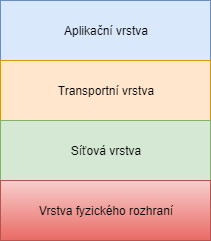
\includegraphics{obrazky/TCP_IP.png}}
    \caption{Architektura TCP/IP.}
    \label{img:architektura_tcpip}
\end{figure}

\section{Vrstva fyzického rozhraní}
Jedná se o~nejnižší vrstvu v~TCP/IP modelu a~má na starost přenos rámců mezi dvěma zařízeními. Tato vrstva popisuje, jakým způsobem dochází k~přístupu na fyzické médium, jako jsou například koaxiální kabely a~optické vlákna.

Tato vrstva není nijak blíže specifikované, protože záleží na použité přenosové technologie. Tou může být Ethernet, Token Ring, telefonní linka X.25 a~další. Nezávislosti síťové vrstvy na nějaké konkrétní technologii umožňuje architektuře TCP/IP rychlou adaptaci na nové technologie. Dnes nejznámější a~nejpoužívanější přenosová technologie je Ethernet.

Fyzická zařízení na této vrstvě jsou identifikovaná pomocí MAC adresy. Jedná se o~48 bitovou adresu, zapisovanou šesticí dvojciferných hexadecimálních čísel oddělená dvojtečkou. Každému zařízení je MAC adresa přidělena při výrobě.

\subsection{Ethernet}
Tento protokol zapouzdřuje data do rámců. Rámce jsou tvořeny tzv. preambulí, ethernetovou hlavičkou, samotnými daty a~kontrolním součtem. Formát ethernetového rámce je znázorněn na obrázku \ref{img:hlavika_ethernet}.

\begin{figure}[H]
    \centering
    \scalebox{0.5}{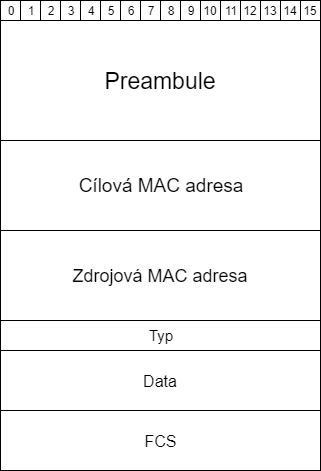
\includegraphics{obrazky/Ethernet.png}}
    \caption{Ethernetový rámec}
    \label{img:hlavika_ethernet}
\end{figure}

Popis položek ethernetového rámce:

\begin{itemize}
    \item \textbf{Preambule} - slouží k synchronizaci hodin příjemce;
    \item \textbf{Cílová MAC adresa} - MAC adresa cílového síťového rozhraní;
    \item \textbf{Zdrojová MAC adresa} - MAC adresa zdrojového síťového rozhraní;
    \item \textbf{Typ} - určuje následující protokol;
    \item \textbf{FCS} - cyklický redundantní součet, umožňující odhalení poškození rámce.
\end{itemize}

\section{Síťová vrstva}
Síťová vrstva má na starost vše, co se týká vytváření, adresování a~směrování dat, které se mají přenášet po síti. Přenášená data zabaluje do IP datagramů, které obsahují všechny informace potřebné k~doručení dat na koncovou stanici. Data se snaží doručovat tou nejvhodnější cestou.

Protokoly pracující na síťové vrstvě jsou například IP, ARP, ICMP, IGMP.

\subsection{IPv4}
Internetový protokol verze 4 (IPv4) \cite{ipv4} je nespojovaný protokol nezajišťující spolehlivost, který má na starost adresaci a~směrování datagramů mezi dvěma zařízeními.

Protokol definuje základní jednotku dat, která jsou přenášena na úrovni síťové vrstvy, nazvanou IP datagram. Protokol definuje vnitřní formát těchto datagramů a~další aspekty nespolehlivé a~nespojované služby, jako jsou například podmínky toho, kdy mají být zahazovány pakety, kdy se mají generovat chybová hlášení a~jak mají tato hlášení vypadat.

IPv4 datagramy mohou být při přenášení přes síť fragmentovány do menších částí. K~této fragmentaci dochází, aby bylo možné datagramy přenést přes každou část přenosové trasy. Každá tato část má totiž definovanou svoji maximální přenosovou jednotku (MTU). Tato jednotka určuje maximální velikost IP datagramu, který je možný poslat přes dané síťové rozhraní. 

Hlavička protokolu IPv4 má obvykle 20 bytů a~je znázorněna na obrázku \ref{img:hlavika_ipv4}.

\begin{figure}[H]
    \centering
    \scalebox{0.6}{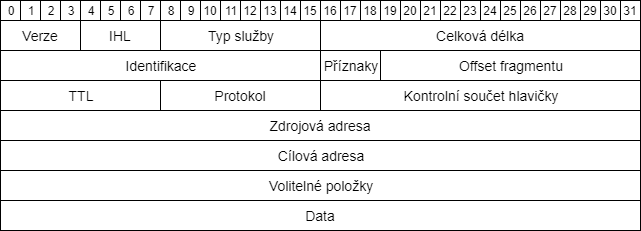
\includegraphics{obrazky/IPv4.png}}
    \caption{Hlavička IPv4.}
    \label{img:hlavika_ipv4}
\end{figure}

Popis položek z~hlavičky protokolu IPv4:

\begin{itemize}
    \item \textbf{Verze} - verze IP, v~tomto případě 4;
    \item \textbf{IHL} - délka hlavičky vyjádřená jako počet bajtů vydělených číslem 4;
    \item \textbf{Typ služby} - toto pole nese značky pro mechanismy zajišťující služby s~definovanou kvalitou (QoS);
    \item \textbf{Celková délka} -  délka IP datagramu (IP hlavička + data);
    \item \textbf{Identifikace} -  jednoznačná identifikátor, sloužící k~identifikaci datagramu, do které patří tento fragment. Každý fragment datagramu má stejný identifikátor;
    \item \textbf{Přiznaky} - celkem tři příznaky, které slouží k~řízení fragmentace;
    \item \textbf{Offset fragmentu} - pozice v~původním datagramu, na které začíná tento fragment;
    \item \textbf{TTL} - délka života datagramu. Jedná se o~ochranu proti zacyklení, pokud dosáhne hodnoty 0, datagram bude zahozen;
    \item \textbf{Protokol} -  určuje protokol, který následuje po IP hlavičce;
    \item \textbf{Kontrolní součet hlavičky} -  kontrolní součet vypočítaný pouze z IP hlavičky;
    \item \textbf{Zdrojová adresa} -  IPv4 adresa odesílatele;
    \item \textbf{Cílová adresa} - IPv4 adresa příjemce.
\end{itemize}

\subsection{IPv6}
Internetový protokol verze 6 (IPv6) \cite{ipv6} dnes nahrazuje již nedostačující protokol IPv4. Hlavním důvodem přechodu z~IPv4 na IPv6 je nedostatek adresovatelných IPv4 adres, které již byly oficiálně vyčerpány roku 2011. Mezi další výhody tohoto protokolu patří zjednodušení při přidělování adres a~zjednodušení přečíslování při změně poskytovatele, kdy stačí na směrovači pouze změnit prefix sítě. 

Hlavička protokolu IPv6 byla oproti protokolu IPv4 změněna. Počet položek v~hlavičce byl zredukován na 8, velikost hlavičky byla nicméně zvýšena o~dvojnásobek na 40 bytů. Hlavním důvodem větší velikosti je velikost zdrojové a cílové adresy, které dohromady mají 32 bytů. Hlavička je znázorněna na obrázku \ref{img:hlavika_ipv6}.

IPv6 může být také rozšířen o~další hlavičky. Tyto hlavičky nazýváme rozšiřující hlavičky. Pokud paket obsahuje rozšiřující hlavičku, je typ rozšiřující hlavičky uveden v~hlavičce IPv6 v~poli, které obsahuje informaci o~následující hlavičce. Každá tato rozšiřující hlavičky má svou vlastní informaci o~následující hlavičce. Rozšiřující hlavičky mohou například sloužit k~směrování, šifrování a~autentizaci. 

\begin{figure}[H]
    \centering
    \scalebox{0.5}{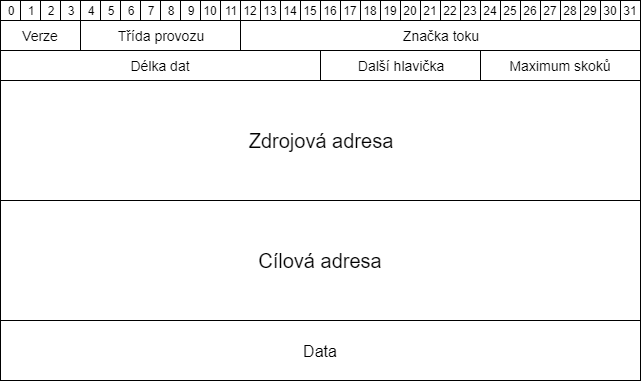
\includegraphics{obrazky/IPv6.png}}
    \caption{Hlavička IPv6.}
    \label{img:hlavika_ipv6}
\end{figure}

Popis položek z~hlavičky protokolu IPv6:

\begin{itemize}
    \item \textbf{Verze} - verze IP, v~tomto případě 6;
    \item \textbf{Třída provozu} - umožňuje specifikovat požadavky na vlastnosti sítě, který daný datagram má;
    \item \textbf{Značka toku} - pomocí značky toku se identifikuje tok, který je chápán jako proud datagramů od stejného odesílatele ke stejnému příjemci se stejnými vlastnosti;
    \item \textbf{Délka dat} - délka přenášených dat;
    \item \textbf{Další hlavička} - určuje typ dat, které následují po IP hlavičce. Může jít buď o~další protokol nebo o~rozšiřující hlavičku.
    \item \textbf{Maximum skoků} - obdoba TTL u~IPv4;
    \item \textbf{Zdrojová adresa} - IPv6 adresa odesílatele;
    \item \textbf{Cílová adresa} - IPv6 adresa příjemce.
\end{itemize}

\section{Transportní vrstva}
Transportní vrstva má na starost přenos dat mezi aplikacemi na zdrojovém a~cílovém počítači. Protokoly transportní vrstvy rozdělují přenášená data na menší části, které se posílají po síti. Tyto části nazýváme pakety. Nejčastějšími příklady protokolů, které pracují na transportní vrstvě, jsou protokoly UDP a~TCP.

\subsection{TCP}
Transmission Control Protocol (TCP) \cite{tcp} je nejpoužívanější protokol transportní vrstvy v~rodině protokolů TCP/IP. Jedná se o~spolehlivou a~spojovanou doručovací službu a~tedy musí byt před výměnou dat mezi klienty ustanoveno spojení. Po ustavení spojení si mohou klienti mezi sebou posílat data v~obou směrech. Spolehlivost protokolu se zajišťuje pomocí číslování jednotlivých segmentů a kontrolou jejich přijetí. Pokud není některý ze segmentů přijat nebo je poškozen, požádá se o~jeho opětovné odeslání. Data se znovu odešlou také, pokud již vypršel čas, kdy měla být přijata zpráva o~doručení dat. Integrita přenášených dat je zajištěna kontrolním součtem.

Pro rozlišování jednotlivých aplikací používá protokol TCP čísla portů. Číslo portu může nabývat hodnot 1 až 65535, přičemž porty 1 až 1023 jsou vyhrazené pro nejběžnější služby. Pokud má nějaká komunikace na síti shodnou pětici údajů a~to cílovou a~zdrojovou IP adresu, cílový a~zdrojový port a~stejný protokol, patří všechny tyto pakety do jednoho síťového toku.

Hlavička protokolu TCP má obvykle 20 bytů a je znázorněna na obrázku \ref{img:hlavika_tcp}. Pro výpočet kontrolního součtu se v~hlavičce používá tzv. pseudohlavička. Tato hlavička se pomyslně připojí k~vlastnímu datagramu, avšak není ve skutečnosti odesílatelem k~příjemci odesílána. Pseudohlavička obsahuje IP adresy odesílatele a~příjemce, identifikátor protokolu a~velikost datagramu bez této pseudohlavičky. 

\begin{figure}[H]
    \centering
    \scalebox{0.6}{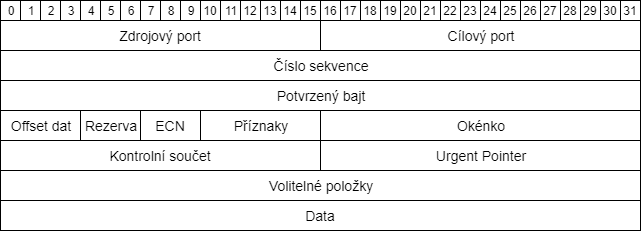
\includegraphics{obrazky/TCP.png}}
    \caption{Hlavička TCP.}
    \label{img:hlavika_tcp}
\end{figure}

Popis položek z~hlavičky protokolu TCP.

\begin{itemize}
    \item \textbf{Zdrojový port} - číslo zdrojového portu;
    \item \textbf{Cílový port} - číslo cílového portu;
    \item \textbf{Číslo sekvence} - pořadové číslo prvního datového bytu v~tomto segmentu;
    \item \textbf{Potvrzený bajt} - hodnota dalšího pořadového čísla, který odesílatel očekává;
    \item \textbf{Offset dat} - označení, kde začínají data;
    \item \textbf{Okénko} - množství dat v~bajtech, které je potvrzováno najednou;
    \item \textbf{Kontrolní součet} vypočítaný kontrolní součet z~TCP datagramu a~pseudohlavičky;
\end{itemize}

\subsection{UDP}
 User Datagram Protocol (UDP) \cite{udp} je doručovací služba, běžící na transportní vrstvě. Na rozdíl od protokolu TCP, je UDP nespojovaná a nespolehlivá služba. UDP tedy před výměnou nenavazuje spojení a~nijak nekontroluje, zda-li vůbec a~v~jakém pořadí byly data doručeny.

Stejně jako protokol TCP i~UDP používá pro rozlišování jednotlivých aplikací čísla portů. Protokol UDP má svoji vlastní sadu portů, které jsou nezávislé. Hlavička je oproti protokolu TCP menší. V~hlavičce se přenášejí pouze informace o~zdrojovém a~cílovém portu, délka UDP paketu včetně dat a~kontrolní součet. Stejně jako u~protokolu TCP, i~zde se pro výpočet kontrolního součtu používá pseudohlavička. Velikost hlavičky je 8 bytů a~je znázorněna na obrázku \ref{img:hlavika_udp}. 

\begin{figure}[H]
    \centering
    \scalebox{0.6}{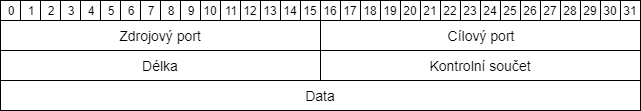
\includegraphics{obrazky/UDP.png}}
    \caption{Hlavička UDP.}
    \label{img:hlavika_udp}
\end{figure}

Popis položek UDP hlavičky:

\begin{itemize}
    \item \textbf{Zdrojový port} - číslo zdrojového portu;
    \item \textbf{Cílový port} - číslo cílového portu;
    \item \textbf{Délka} - délka UDP datagramu (UDP hlavička + data);
    \item \textbf{Kontrolní součet} - vypočítaný kontrolní součet z~UDP datagramu a~pseudohlavičky. 
\end{itemize}

\section{Aplikační vrstva}
Aplikační vrstvu tvoří procesy a~aplikace, které komunikují po síti. Tyto procesy a~aplikace definují protokoly, které používají k~výměně dat. Většina protokolů aplikační vrstvy vychází z~modelu klient/server. Klient žádá o~konkrétní služby a~je iniciátorem veškeré komunikace, zatímco server poskytuje své služby pouze na základě žádosti klienta. Způsob komunikace mezi klientem a~serverem si určuje každý protokol sám. Tato vrstva je z~hlediska této práce nepodstatná. 

Na aplikační vrstvě pracuje velké množství protokolů. Mezi nejznámější patří například protokoly FTP, POP3, DHCP, BitTorrent, IMAP a další. 

\chapter{Zachytávání a zpracování dat}
\label{chap:zachyt}
Tato kapitole je zaměřená na způsoby zachytávání paketů na síti a~práci s~nimi. V~této kapitole představím základní metody, jakými se dají zachytávat data na síti a~na způsoby zpracování již zachycených dat, respektive na aplikaci, která k~tomuto účelu slouží. Informace uvedené v~této kapitole jsou volně přejaty z~knihy \emph{Practical Packet Analysis} \cite{analyza}.

\section{Zachytávání dat}
Existuje několik způsobů jak zachytávat pakety, které jsou přenášeny přes síť. V~této kapitole jsou popsaný dva nejpoužívanější způsoby zachytávání paketů v~síti a~to zrcadlení portu a~síťový odposlech. 

Pro zachytávání paketů v~síti je nutné vlastnit síťovou kartu, která umožňuje přechod do promiskuitního režimu. V promiskuitním režimu dokáže síťová karta zachytávat všechny data, která procházejí sítí. V dnešní době umožňují přechod do promiskuitního režimu téměř všechny síťově karty. Jediná situace, kdy nepotřebujeme mít přepnutou kartu v~promiskuitním režimu, je situace, kdy chceme sledovat komunikaci pouze na našem zařízení.

Síťová karta, která není v promiskuitním režimu, přijímá pouze data, která jsou určena pro její MAC adresu nebo pokud jde o~zprávy typu broadcast či multicast. Zprávy typu broadcast jsou totiž posílány všem účastníkům v~dané síti. Zprávy typu multicast jsou zase posílány všem účastníkům dané multicastové skupiny.

\subsection{Zrcadlení portu}
Zrcadlení portu je asi nejjednodušší způsob zachytávání provozu cílového zařízení na síti. Zrcadlení portu se musí nastavit v~rozhraní přepínače a~přepínač jej musí podporovat. Pro použití zrcadlení portu je také nutné mít na přepínači ještě jeden volný port, kam lze připojit sledovací zařízení.

Při konfiguraci zrcadlení portu se nastaví, který port bude zrcadlen na určitý port. Na tento port se potom připojí sledovací zařízení. Sledovací zařízení poté může vidět všechny pakety, které zařízení, připojené k~zrcadlenému portu, přijímá i~odesílá. 

\subsection{Zařízení \uv{tap}}
Zařízení \uv{tap} je zařízení, které se umístí mezi dva body v~kabeláži, kde chceme zachytávat pakety. Jedná se o~speciální zařízení, určené k~zachytávání paketů.

Existují dva typy těchto zařízení a~to agregované a~neagregované. Hlavní rozdíl mezi těmito typy je počet portů. Agregované zařízení mají porty 3, neagregované 4. Neagregované zařízení mají na rozdíl od agregovaných 2 monitorovací porty. Jeden monitorovací port slouží pro odposlouchávání komunikace v~jednom směru a~druhý port pro odposlouchávání komunikace v~opačném směru. Agregované zařízení mají pouze jeden monitorovací port, který slouží k~zachytávání paketů v~obou směrech. 

\subsection{PCAP soubory}
Soubory typu PCAP jsou datové soubory se zachycenou síťovou komunikací. Jedná se o~nejběžnější formát, do kterého se ukládá zachycená síťová komunikace.

PCAP soubory vždy začínají globální hlavičkou, za kterou následuje 0 nebo více záznamů pro každý zachycený paket. Struktura této globální hlavičky je znázorněna ve výpise \ref{list:global}. Záznam paketu obsahuje hlavičku paketu, obsahující základní informace o~paketu, a~samotná zachycená data paketu. Struktura hlavičky paketu je znázorněna ve výpise \ref{list:paket}. Formát souboru PCAP je znázorněn na obrázku \ref{img:pcap}.

\begin{figure}[H]
    \centering
    \scalebox{0.7}{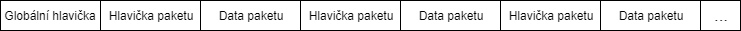
\includegraphics{obrazky/PCAP.png}}
    \caption{Formát souboru PCAP}
    \label{img:pcap}
\end{figure}

Struktura globální hlavičky:

\begin{lstlisting}[style=npl, caption={Struktura globální hlavičky}, label={list:global}]
typedef struct pcap_hdr_s {
    guint32 magic_number;   /* Magické číslo */
    guint16 version_major;  /* Hlavní číslo verze */
    guint16 version_minor;  /* Vedlejší číslo verze */
    gint32  thiszone;       /* Korekce lokální času ku GMT */
    guint32 sigfigs;        /* Přesnost časového razítka */
    guint32 snaplen;        /* Maximální velikost zachycených paketů v~bajtech */
    guint32 network;        /* Typ síťového zařízení */
} pcap_hdr_t;
\end{lstlisting}

Struktura hlavičky paketu:

\begin{lstlisting}[style=npl, caption={Struktura hlavičky paketu}, label={list:paket}]
typedef struct pcaprec_hdr_s {
    guint32 ts_sec;         /* Sekundy časového razítka*/
    guint32 ts_usec;        /* Mikrosekundy časového razítka */
    guint32 incl_len;       /* Velikost paketu uloženého v~souboru v~bajtech */
    guint32 orig_len;       /* Skutečná délka paketu */
} pcaprec_hdr_t; 
\end{lstlisting}

\section{Zpracování dat}
Tato část popisuje aplikace, které slouží k~analýze zachycených paketů. K~práci se zachycenými daty jsem používal aplikaci Wireshark a~její odnož TShark. 

\subsection{Wireshark}
Wireshark je aplikace určená pro zachytávání a~analýzu paketů. Aplikace je multiplatformní a~nabízí přehledné uživatelské rozhraní. Wireshark dokáže analyzovat zachycenou síťovou komunikaci do nejmenších detailů a~vytvářet různé statistiky a~data. Wireshark dále umožňuje přepnout kartu do promiskuitního režimu, aby uživatel mohl sledovat všechny pakety, kterou tečou v~síti. Zachycené pakety lze také ukládat do několik různých formátu, z~nichž nejčastější jsou PCAP soubory.

Wireshark dnes podporuje více jak 850 různých protokolů a~každou aktualizací přibývají další nové protokoly. Nesmírnou výhodou je otevřený zdrojový kód. Díky tomu může přidávat podporu nějakého protokolu prakticky každý, kdo má patřičné programátorské schopnosti. Vzhled aplikace je zobrazen na obrázku \ref{img:wireshark}.

\begin{figure}[H]
    \centering
    \scalebox{0.6}{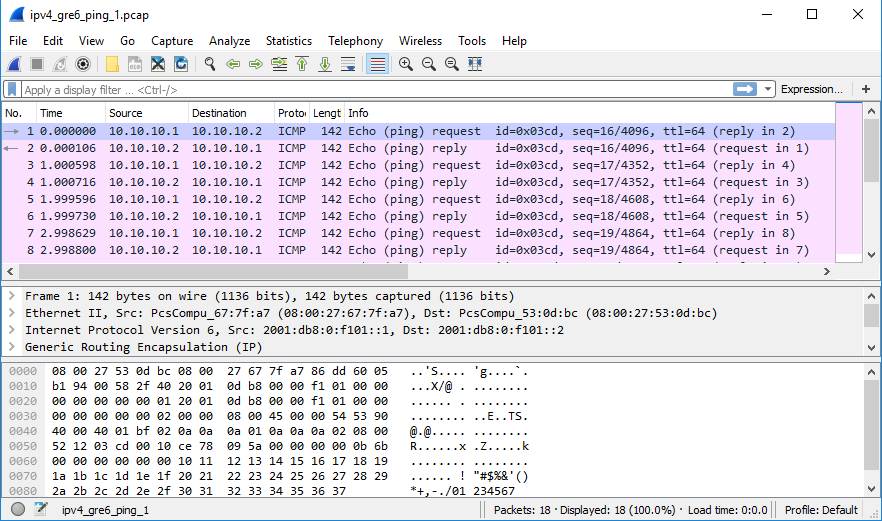
\includegraphics{obrazky/wireshark.png}}
    \caption{Vzhled aplikace Wireshark}
    \label{img:wireshark}
\end{figure}

\subsection{TShark}
TShark je odlehčená verze Wiresharku, která neobsahuje uživatelské rozhraní. Tato aplikace se tedy ovládá pouze přes příkazový řádek. Tato verze nabízí podobnou funkcionalitu jako Wireshark, s~tím, že některé funkce nejsou díky chybějícímu uživatelskému rozhraní dostupná. Umožňuje tedy například zachytávání paketů na síťovém rozhraní, čtení PCAP souborů a~ukládání zachycené komunikace do různých souborových formátů. Aplikace je ovládána pomocí přepínačů z~příkazové řádky.

\subsection*{Příklady použití}
Příklad příkazu pro zachytávání paketů:
\begin{lstlisting}[language=bash]
    $ tshark -i sitove_zarizeni -w nazev_souboru.pcap 
\end{lstlisting}
Příkaz pro čtení PCAP souboru:
\begin{lstlisting}[language=bash]
    $ tshark -r nazev_souboru.pcap 
\end{lstlisting}
Příklad příkazu pro převod PCAP souboru do formátu PDML (XML)
\begin{lstlisting}[language=bash]
    $ tshark -r nazev_souboru.pcap -T pdml > vystup.pdml
\end{lstlisting}

\chapter{Tunelovací protokoly}
\label{chap:tunel}
Pojmem tunelování se v počítačových sítí rozumí situace, kdy jsou pakety jednoho síťového protokolu vkládány jako data do jiného síťového protokolu. Tunelování umožňuje například přenášet data přes nekompatibilní sítě, obcházet některá administrativní omezení sítě a~poskytovat zabezpečené spojení přes nezabezpečenou síť. Základní princip tunelování je zobrazen na obrázku \ref{img:tunel}.

Tunelovací protokoly fungují na principu zapouzdření datové části paketu tunelovaného protokolu do protokolu jiného. Při tunelování obvykle dojde k narušení pořadí vrstev, protože se data některé vrstvy modelu zapouzdřují do protokolu, běžící na stejné nebo vyšší vrstvě.

\begin{figure}[H]
    \centering
    \scalebox{1.0}{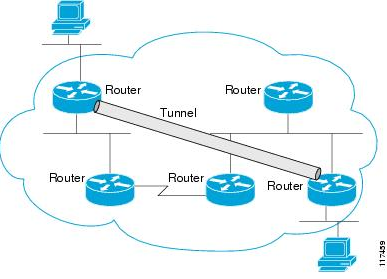
\includegraphics{obrazky/tunelovani.png}}
    \caption{Základní princip tunelování. Na obrázku je znázorněn princip vytvoření tunelu mezi dvěma směrovači.}
    \label{img:tunel}
\end{figure}

\section{GRE}
Generic Routing Encapsulation (GRE) \cite{gre} je tunelovací protokol, který pracuje na síťové vrstvě. Protokol byl vyvinutý společností Cisco~a umožňuje zapouzdření velké škály protokolů síťově vrstvy uvnitř virtuální přímého spojení přes IP protokol.

GRE zapouzdřuje užitečná data, vnitřní paket určený k doručení, do vnějšího paketu. Ten se poté pošle skrz GRE tunel. Mezilehlé routery jej směrují jako vnější paket, takže jej předají do cílové sítě, kde je vnější paket odebrán a~původní paket je směrován ke svému cíli.

GRE protokol poskytuje bezstavové privátní spojení, které je ovšem nezabezpečené. Protokol GRE totiž sám o~sobě nepoužívá žádné šifrování dat.

Při použití GRE tunelu přidáme do paketu dvě hlavičky. První přidanou hlavičkou je vnější IP hlavička, která je vložena před původní IP hlavičku. Mezi ně je poté vložena GRE hlavička. Standardní velikost GRE hlavičky bez volitelných položek jsou 4 byty. Hlavička je znázorněna na obrázku \ref{img:hlavicka_gre}.

Protokol GRE definuje celkově dvě verze hlaviček. První verze, verze 0, je určena pro klasický samotný GRE tunel. Druhá verze, verze 1, je určena pro protokol PPTP, o~kterém pojednává kapitola \ref{sec:pptp}.

\begin{figure}[H]
    \centering
    \scalebox{0.6}{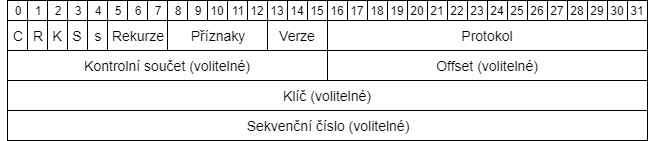
\includegraphics{obrazky/GRE.png}}
    \caption{GRE hlavička, verze 0}
    \label{img:hlavicka_gre}
\end{figure}

Popis vybraných položek GRE hlavičky:

\begin{itemize}
    \item \textbf{C, R, K, S} - příznaky, které udávají informace o~tom, zda se v~hlavičce nachází dané volitelné položky;
    \item \textbf{Rekurze} - obsahuje údaj o~tom, kolik dalších zapouzdření je povoleno;
    \item \textbf{Příznaky} - rezervované bity, musí byt nastaveny na 0.
    \item \textbf{Verze} - verze GRE hlavičky. 1, pokud se jedná o~protokol PPTP, jinak 0;
    \item \textbf{Protokol} - protokol, který je protokolem GRE zapouzdřen;
    \item \textbf{Kontrolní součet} - vypočítaný kontrolní součet z~GRE hlavičky a~dat;
    \item \textbf{Klíč} - obsahuje číslo, které bylo vloženo společně se zapouzdřením. Přijímací strana je může použít k~ověření zdroje paketu;
    \item \textbf{Sekvenční číslo} - obsahuje číslo, které bylo vloženo společně se zapouzdřením. Přijímací strana je může použít k~určení pořadí, v~jaké byly pakety byly pakety odeslány.
\end{itemize}

\section{IPIP}
IP in IP (IPIP) je tunelovací protokol, který zapouzdřuje IP paket jiným IP paketem. Po zapouzdření se přidá nová IP hlavička, která bude mít odlišené hodnoty zdrojové a~cílové adresy. V~těchto adresách je uveden vstupní a~výstupní bod tunelu.

IPIP tunel je možné realizovat libovolnou kombinací IP protokolů. IPv4 protokol může zapouzdřovat IPv6 protokol, stejně tak i~naopak. Možné je i~zapouzdřovat IP protokol stejným typem IP protokolu. Způsob, jakým jsou dat zapouzdřena je znázorněn na obrázku \ref{img:ipip}.

\begin{figure}[H]
    \centering
    \scalebox{0.7}{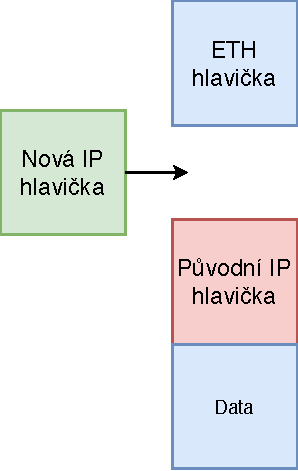
\includegraphics{obrazky/IPIP.png}}
    \caption{IPIP zapouzdření}
    \label{img:ipip}
\end{figure}

\section{PPTP}
\label{sec:pptp}
Point-to-Point Tunneling Protocol (PPTP) \cite{pptp} je metoda pro realizaci virtuálních privátních sítí (VPN). Protokol pro řízení používá protokol TCP a pro zapouzdření PPP paketů používá protokol GRE.

PPTP používá ke komunikace ve výchozím nastavení TCP spojení na portu 1723. Toto spojení je používáno k~iniciování a~řízení GRE tunelu. PPTP používá pro tunelování pomocí GRE nestandardní upravenou verzi hlavičky. Do hlavičky byly zavedeny nové položky potvrzovací číslo, id volání a~délka dat. Do hlavičky také přibyl jeden příznak, pro indikaci, zda je v~hlavičce potvrzovací číslo uvedeno. Z~hlavičky naopak ubyly informace o~kontrolním součtu, klíč a~offset. Hlavička samotného protokolu PPTP, která se používá při iniciování a~řízení spojení, je zobrazena na obrázku \ref{img:hlavicka_pptp}. 

\begin{figure}[H]
    \centering
    \scalebox{0.6}{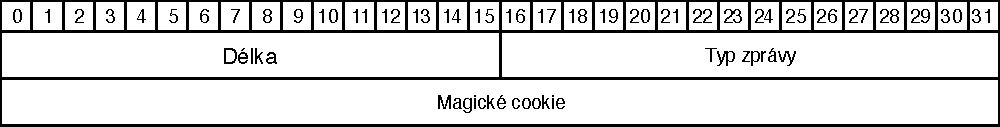
\includegraphics{obrazky/PPTP.png}}
    \caption{PPTP hlavička}
    \label{img:hlavicka_pptp}
\end{figure}

Popis položek z~hlavičky PPTP:

\begin{itemize}
    \item \textbf{Délka} - velikost PPTP zprávy v~bytech;
    \item \textbf{Typ zprávy} - může nabývat hodnot 1 nebo 2. Zprávy typu 2 nicméně nejsou definovány;
    \item \textbf{Magické cookie} - hodnota tohoto pole je vždy nastavena na 0x1A2B3C4D.
\end{itemize}

\section{L2TP}
Layer 2 Tunneling Protocol (L2TP) \cite{l2tpv2} je tunelovací protokol, určený k~použití pro podporu VPN. Tento protokol má původ ve dvou starších tunelovacích protokolech. Vychází z~protokolů Layer 2 Forwarding Protocol (L2F) a~z~protokolu PPTP.

Celý L2TP paket je odeslán v~rámci datagramu UDP. Protokol sám o~sobě neposkytuje žádné šifrování ani zabezpečení. Z~toho důvodu se často používá ve spolupráci s~protokolem IPsec, který tyto vlastnosti zajišťuje. Tato kombinace protokolů se nazývá L2TP/IPsec. Hlavička protokolu je zobrazena na obrázku \ref{img:l2tpv2}.

\begin{figure}[H]
    \centering
    \scalebox{0.6}{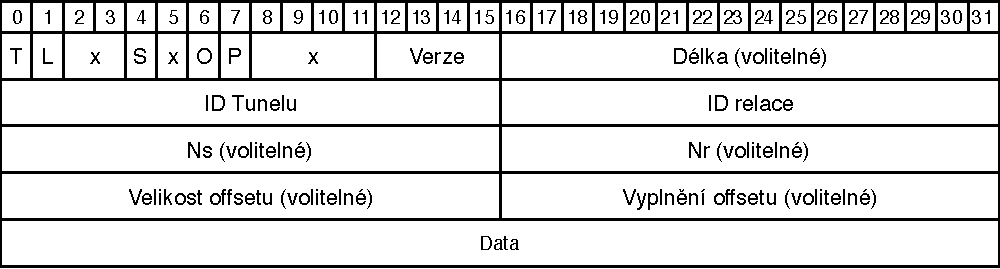
\includegraphics{obrazky/L2TPv2.png}}
    \caption{L2TP hlavička}
    \label{img:l2tpv2}
\end{figure}

Popis položek z~hlavičky L2TP:

\begin{itemize}
    \item \textbf{T, L, x, S, x, O, P} - příznaky a~rezervované bity;
    \item \textbf{Verze} - verze protokolu;
    \item \textbf{Délka} - velikost zprávy v~bajtech;
    \item \textbf{ID tunelu} - jednoznačný identifikátor tunelu pro řízení spojení;
    \item \textbf{ID relace} - jednoznačný identifikátor relace v~tunelu.
    \item \textbf{Ns} - pořadové číslo pro data nebo řídící zprávu.
    \item \textbf{Nr} - pořadové číslo, které je očekávané v~příští řídící zprávě, která má být přijata.
    \item \textbf{Velikost offsetu} - určuje počet bajtů za L2TP hlavičkou, kde se očekává začátek užitečných dat.
    \item \textbf{Vyplnění offsetu} - vyplnění pole offsetu do velikost 32 bitů.
\end{itemize}

V~roce 2005 byla vydána nová verze protokolu L2TPv3 \cite{l2tpv3}. Tato verze přinesla nové zabezpečovací funkce, upravené zapouzdření a~možnost přenášet data přes jiné sítě, než přes sítě IP. Dále přibyla možnost zapouzdřit pouze protokol IP bez nutnosti zapouzdření UDP.

\chapter{Dataset}
\label{chap:dataset}
Pro získávání tunelovaných dat bylo nutné vytvořit prostřední pro jejich získávání. K~tomuto účelu jsem potřeboval vhodné testovací prostředí. Rozhodl jsem, že toto prostředí bude virtualizované. Na vytváření virtuálních počítačů jsem použil aplikaci Oracle VM VirtualBox. Celkem jsem pro vytváření dat využil tři virtuální stroje. Dva stroje byly využity k~vytváření tunelů a~jeden stroj byl využit k~monitorování sítě. Monitorování sítě bylo prováděno pomocí aplikace Wireshark a~zachycená síťová komunikace zde také byla ukládaná do PCAP souborů. Testovací topologie je znázorněna na obrázku \ref{img:topologie}. Všechny tři virtuální stroje využívali operační systém Linux, konkrétně linuxuvou distribuci Ubuntu. V~části \ref{sec:nastroje} jsou popsané nástroje, které jsem pro vytváření testovacích dat využíval. V~části \ref{sec:prostredi} je popsáno prostředí, ve kterém byly testovací data vytvářena.

\begin{figure}[H]
    \centering
    \scalebox{0.6}{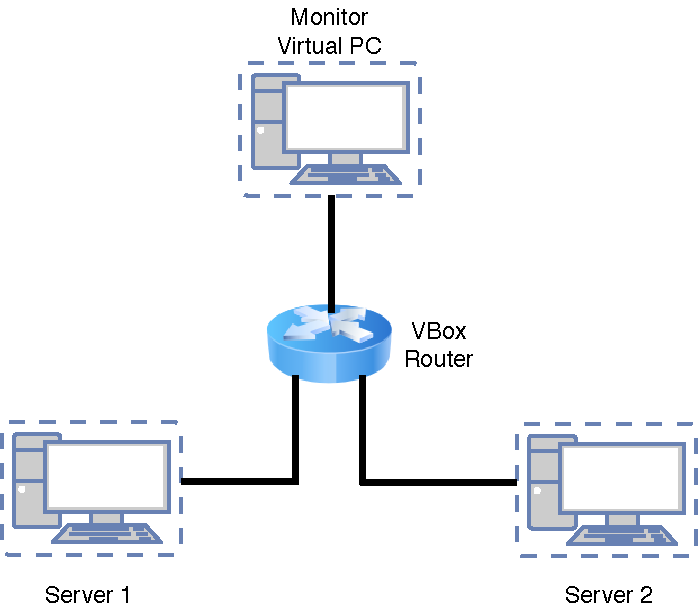
\includegraphics{obrazky/Topologie.png}}
    \caption{Testovací topologie}
    \label{img:topologie}
\end{figure}

\section{Nástroje}
\label{sec:nastroje}
Tato část popisuje nástroje použité pro získávání testovacích dat. Pro tento účel bylo nutné použít nástroje pro vytváření a~spouštění virtuálních strojů. K~tomuto účelu jsem využil aplikaci jménem VirtualBox. Dále byly potřebné nástroje pro vytváření tunelů mezi stroji. Na to jsem využíval nástroje z~balíčku nástrojů jménem \emph{iproute2}.

\subsection{Oracle VM VirtualBox}
\emph{VirtualBox} byl původně vyvinutý německou společností Innotek GmbH. Tuto společnost však v~roce 2008 odkoupila společnost Sun Microsystems, kterou vzápětí v~roce 2009 odkoupila společnost Oracle. 

Jedná se o~nástroj určený k~virtualizaci operačních systémů. Aplikace je multiplatformní a~je určena pro operační systémy Windows, Linux/Unix i~Mac OS.

\subsection{iproute2}
\emph{Iproute2} je balíček nástrojů pro ovládání a~monitorování různých aspektů sítí v~Linuxovém jádře, jako jsou například směrování, síťové rozhraní, tunely, a~tak dále. Tento balíček obsahuje několik nástrojů, mezi nejvýznamnější nástroje patří \emph{ip} a~\emph{tc}. Nástroj \emph{ip} slouží ke konfiguraci IPv4 a IPv6 sítí, zatímco nástroj \textit{tc} slouží k~ovládání síťového provozu.

Cílem balíčku \emph{iproute2} je nahradit starší balík nástrojů \emph{net-tools}, které již nejsou dále vyvíjeny. Všechny nástroje obsahují detailní informace a~dokumentaci. Jak byly nástroje z~balíčku \emph{net-tools} nahrazeny nástroji z~balíčku \emph{iproute2} je ukázáno v~tabulce \ref{tab:iproute2}.

\begin{table}[H]
    \centering
    \begin{tabular}{| c | c | c |}
        \hline
         \textbf{Účel} & \textbf{net-tools} & \textbf{iproute2}  \\
         \hline
         Konfigurace dat a spojení & ifconfig & ip addr, ip link \\
         \hline
         Směrovací tabulky & route & ip route \\
         \hline
         Sousedé & arp & ip neight \\
         \hline
         VLAN & vconfig & ip link \\
         \hline
         Tunely & iptunnel & ip tunnel \\
         \hline
         Multicast & ipmaddr & ip maddr \\
         \hline
         Statistiky & nestat & ss \\
         \hline
    \end{tabular}
    \caption{Nahrazení nástrojů \emph{net-tools} nástroji \emph{iproute2}}
    \label{tab:iproute2}
\end{table}

Jak lze vidět z~tabulky, pro vytváření tunelů jsem tedy využíval nástroj \emph{ip tunnel}. Tunely jsem vytvářel pomocí následujícího příkazu:

\begin{lstlisting}[language=bash]
    $ ip tunnel add NAZEV mode MOD remote ADRESA local ADRESA
\end{lstlisting}
, kde:

\begin{DESCRIPTION}
    \item[NAZEV] Je název síťového rozhraní, reprezentující tunel
    \item[MOD] Je typ tunelu, který chceme vytvořit
    \item[ADRESA] IP adresa
\end{DESCRIPTION}
Kompletní popis tohoto příkazu lze nalézt na jeho manuálových stránkách \cite{iptunnel}.

Virtuální stroje \emph{Server 1} a~\emph{Server 2} byly použity k~vytváření tunelů. Tunely jsem vytvářel právě mezi těmito dvěma stroji. Třetí stroj, nazvaný \emph{Monitor Virtual PC}, jsem používal k~zachytávání paketů na sítí. Zachytávání paketů jsem prováděl pomocí aplikace Wireshark a~síťové karty, která byla přepnutá do promiskuitního režimu.

\section{Prostředí}
\label{sec:prostredi}
Všechny virtuální stroje obsahovali operační systém Ubuntu ve verzi 16.04.03. Jedná se o~linuxuvou distribuci, určenou pro laptopy, stolní počítače i~servery. Jde o~komunitně vytvářený operační systém, zastřešený britskou společností \emph{Canonical}. Systém je distribuován zcela zdarma.

Stroje, které byli použity k~vytváření tunelů, používaly Ubuntu ve verzi \emph{Server}. Tato verze Ubuntu nenabízí žádné uživatelské prostředí, pouze příkazoví řádek a~obsahuje řadu užitečných nástrojů, určených pro administrátory. Bylo tak učiněno z~důvodů omezeného výkonu na mém fyzickém počítači a~z~důvodu, že tyto virtuální stroje uživatelské rozhraní vůbec nepotřebovaly. Poslední virtuální stroj, určený k~zachytávání paketů, už používal klasickou verzi Ubuntu s~uživatelským rozhraním. Na tomto stroji již bylo uživatelské rozhraní nutné, protože na něm běžela aplikace Wireshark. 

\chapter{Návrh extraktoru}
\label{chap:navrh}
Tato kapitola se věnuje návrhu aplikace, která je cílem této bakalářské práce. Návrh aplikace je rozdělen do několika jednotlivých částí. Celkem je těchto částí 5 a~každá část zastává jinou činnost při extrakci tunelovaných dat. Základní princip aplikace a~její části jsou znázorněny na obrázku \ref{img:hlavni}.

\begin{figure}[H]
    \centering
    \scalebox{0.6}{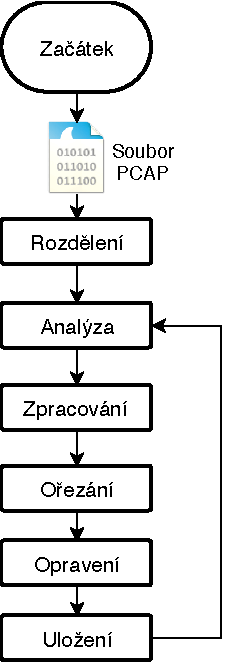
\includegraphics{obrazky/Program.png}}
    \caption{Hlavní část programu. Aplikace je rozdělena na 5 částí. Po rozdělení vstupního souboru na jednotlivé toky, se bude každý takový soubor zpracovávat samostatně.}
    \label{img:hlavni}
\end{figure}

Vstupem aplikace je PCAP soubor. První věc, kterou bude aplikace s~daným souborem provádět je rozdělení souboru na jednotlivé zachycené síťové toky do samostatných PCAP souborů. Činnost této části aplikace je popsána v~části \ref{sec:predzpracovani}. Po rozdělení souboru se bude každý síťový tok zpracovávat samostatně. Každý takový PCAP soubor projde analýzou, kde se bude zjišťovat, zda daný síťový tok je tunelovaný. Činnost analyzátoru je popsána v~části \ref{sec:analyzator}. Pokud analyzátor detekuje tunelovaný provoz, daný PCAP se zpracuje, tzn. dojde k~označená částí, které se mají z~paketu odstranit. Tomuto procesu se věnuje část \ref{sec:zpracovani}. Samotný proces odstraňování částí paketu je popsán v~části \ref{sec:orezavani}. 

Po odstranění některých dat z~paketů se můžou ve zbývajících částech paketu vyskytovat chyby v~hlavičkách. Může jít například o~již neplatný kontrolní součet a~špatnou informaci o~následující hlavičce. Tyto chyby je nutné opravit. Způsob opravování je popsán v~části \ref{sec:opravovani}. Po každém odstraněném zapouzdření se vytvoří nový PCAP soubor, obsahující datový tok bez daného zapouzdření. Takto nově vytvořený soubor se opět zanalyzuje pro případ, že původní soubor obsahoval více zapouzdření. Aplikace tedy bude z~PCAP souboru postupně odstraňovat zapouzdření a~vytvářet nové PCAP soubory.

\section{Přidávání a odebírání vrstev}
Cílem této práce je extrakce tunelovaného provozu. Tohoto cíle se dosáhne za pomocí odstraňování různých vrstev v~paketu. Při odstranění některé vrstvy ale můžeme narazit na několik problémů. Vrstvy modelu jsou totiž vzájemně propojeny a~odstraněním některé z~nich může porušit správnost informací v~ostatních vrstvách. Typické informace, které již nemusí při odstranění platit jsou například délka datagramu, následující protokol a~kontrolní součet. Po odstranění některé vrstvy z~paketu je nutné tyto informace změnit, aby tyto informace byli i~nadále konzistentní.

Ke stejné situaci bude docházet i~v~případě, že se rozhodneme do paketu vrstvy naopak přidávat. Při přidávání vrstvy je také nutné u~dané přidávané vrstvě uvádět správné informace o~následujícím protokolu a~případně délky paketu a~kontrolního součtu. 

\section{Předzpracování}
\label{sec:predzpracovani}
Předzpracování je první věc, která se provede se vstupním PCAP souborem. Cílem této části aplikace je rozdělit PCAP soubor, který je vstupem programu, do více PCAP souborů. Soubor bude rozdělen tak, aby každý síťový tok byl v~samostatném souboru. Každý takto vytvořený soubor se poté bude zpracovávat samostatně.

Tato část aplikace bude procházet vstupní soubor paket po paketu a~jednotlivé pakety přidělovat k~daným síťovým tokům. Každý takto oddělený síťový tok se poté bude zpracovávat samostatně. Vstupem této části aplikace je PCAP soubor, který je zároveň vstupem celé aplikace. Výstupem bude \emph{1 až N} PCAP souborů, v~závislosti na počtu síťových toků, které vstupní soubor obsahuje. Základní princip této části aplikace je znázorněn na obrázku \ref{img:predzpracovani}.

\begin{figure}[H]
    \centering
    \scalebox{0.6}{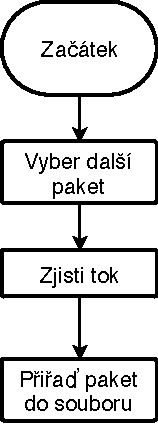
\includegraphics{obrazky/Predzpracovani.png}}
    \caption{Předzpracování. Zde se provádí rozdělení vstupního souboru na menší části, kdy bude každý síťový tok uložen v~jednom souboru.}
    \label{img:predzpracovani}
\end{figure}

\section{Analyzátor}
\label{sec:analyzator}
Tato část aplikace má na starost hledání zapouzdření. Na vstup této části aplikace přijde PCAP soubor, ve kterém se bude hledat zapouzdření. Pokud dojde k~nalezení zapouzdření, PCAP soubor se bude dále zpracovávat. Dojde také k~určení, jaké zapouzdření se v~daném souboru vyskytuje. Na základě toho se poté vyber správný modul pro zpracování. Pokud v~daném souboru nebude žádné zapouzdření nalezeno, nebude se s~tímto souborem dále pracovat. Základní princip této části aplikace je znázorněn na obrázku \ref{img:analyzator}.

\begin{figure}[H]
    \centering
    \scalebox{0.6}{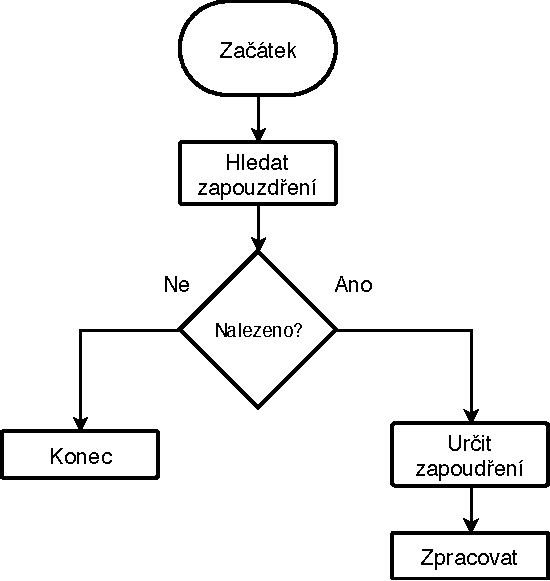
\includegraphics{obrazky/analyzator.png}}
    \caption{Analyzátor. V~této části aplikace se bude hledat v~souboru hledat zapouzdření. Při nalezení zapouzdření se bude soubor dále zpracovávat. }
    \label{img:analyzator}
\end{figure}

\section{Zpracování určitého protokolu}
\label{sec:zpracovani}
Pokud se v~PCAP souboru nalezne zapouzdření, dojde ke zpracování tohoto souboru. V~této části aplikace se pouze označí hlavičky, které mají být z~daného souboru odstraněny. Seznam hlaviček, určených k~odstranění, a~soubor se dále pošlou do funkce, která má ořezávání souboru na starost. 

\section{Ořezávání}
\label{sec:orezavani}
V~této části aplikace se provede ořezání o~dané hlavičky. Vstupem této části je seznam hlaviček, určených k~odstranění, a~soubor. Po odstranění všech označených hlaviček se upravený soubor pošle do funkce, která z~daného souboru odstraní chyby, které mohli vzniknout při odstranění některých hlaviček. 

\section{Opravování}
\label{sec:opravovani}
Při odstranění hlaviček z~paketu může dojít k~chybám v~obsahu u~zbývajících hlaviček hlaviček. Tato část aplikace má za úkol tyto chyby nalézt a~opravit. Typickými chybami, ke kterým může při odstranění hlaviček dojít jsou například informace o~ následující hlavičce a~kontrolní součet. Po opravení těchto chyb se upravený soubor uloží jako nový a~bude znovu poslán k~analýze, jestli neobsahuje další zapouzdření. 

\chapter{Závěr}
Cílem tohoto semestrálního projektu bylo nastudovat síťovou architekturu TCP/IP a~jeho základní protokoly. Dále bylo zapotřebí se seznámit s~tunelovacími protokoly a zaměřit se na možnosti extrakce zapouzdřených dat. Posledním a~hlavním cílem semestrální projektu bylo navrhnout extraktor pro tyto zapouzdřená data.

Dalším cílem této bakalářské práce bude navrženou aplikaci implementovat a~otestovat. Aplikace bude implementována v~programovacím jazyce Python. Pro testování aplikace budou použité již vytvořené testovací soubory. Jedním z~dalších cílů bude nadále vytvářet další testovací soubory pro testování aplikace. Další cílem bude hledání dalších tunelovacích protokolů, aby aplikace podporovala co největší počet tunelovacích protokolů. Aplikace také bude obsahovat snadnou možnost přidávání podpory pro nové tunelovací protokoly. Posledním cíle práce bude provést vyhodnocení funkčnosti aplikace. 

%=========================================================================

  
  % Kompilace po částech (viz výše, nutno odkomentovat)
  % Compilation piecewise (see above, it is necessary to uncomment it)
  %\subfile{projekt-01-uvod-introduction}
  % ...
  %\subfile{chapters/projekt-05-conclusion}


  % Pouzita literatura / Bibliography
  % ----------------------------------------------
\ifslovak
  \makeatletter
  \def\@openbib@code{\addcontentsline{toc}{chapter}{Literatúra}}
  \makeatother
  \bibliographystyle{bib-styles/czechiso}
\else
  \ifczech
    \makeatletter
    \def\@openbib@code{\addcontentsline{toc}{chapter}{Literatura}}
    \makeatother
    \bibliographystyle{bib-styles/czechiso}
  \else 
    \makeatletter
    \def\@openbib@code{\addcontentsline{toc}{chapter}{Bibliography}}
    \makeatother
    \bibliographystyle{bib-styles/englishiso}
  %  \bibliographystyle{alpha}
  \fi
\fi
  \begin{flushleft}
  \bibliography{xnahal01-20-literatura-bibliography}
  \end{flushleft}

  % vynechani stranky v oboustrannem rezimu
  % Skip the page in the two-sided mode
  \iftwoside
    \cleardoublepage
  \fi

  % Prilohy / Appendices
  % ---------------------------------------------
  \appendix
\ifczech
  \renewcommand{\appendixpagename}{Přílohy}
  \renewcommand{\appendixtocname}{Přílohy}
  \renewcommand{\appendixname}{Příloha}
\fi
\ifslovak
  \renewcommand{\appendixpagename}{Prílohy}
  \renewcommand{\appendixtocname}{Prílohy}
  \renewcommand{\appendixname}{Príloha}
\fi
%  \appendixpage

% vynechani stranky v oboustrannem rezimu
% Skip the page in the two-sided mode
%\iftwoside
%  \cleardoublepage
%\fi
  
\ifslovak
%  \section*{Zoznam príloh}
%  \addcontentsline{toc}{section}{Zoznam príloh}
\else
  \ifczech
%    \section*{Seznam příloh}
%    \addcontentsline{toc}{section}{Seznam příloh}
  \else
%    \section*{List of Appendices}
%    \addcontentsline{toc}{section}{List of Appendices}
  \fi
\fi
  \startcontents[chapters]
  \setlength{\parskip}{0pt}
  % seznam příloh / list of appendices
  % \printcontents[chapters]{l}{0}{\setcounter{tocdepth}{2}}
  
  \ifODSAZ
    \setlength{\parskip}{0.5\bigskipamount}
  \else
    \setlength{\parskip}{0pt}
  \fi
  
  % vynechani stranky v oboustrannem rezimu
  \iftwoside
    \cleardoublepage
  \fi
  
  % Přílohy / Appendices
  % Tento soubor nahraďte vlastním souborem s přílohami (nadpisy níže jsou pouze pro příklad)
% This file should be replaced with your file with an appendices (headings below are examples only)

% Umístění obsahu paměťového média do příloh je vhodné konzultovat s vedoucím
% Placing of table of contents of the memory media here should be consulted with a supervisor
%\chapter{Obsah přiloženého paměťového média}

%\chapter{Manuál}

%\chapter{Konfigurační soubor} % Configuration file

%\chapter{RelaxNG Schéma konfiguračního souboru} % Scheme of RelaxNG configuration file

%\chapter{Plakát} % poster
  
  % Kompilace po částech (viz výše, nutno odkomentovat)
  % Compilation piecewise (see above, it is necessary to uncomment it)
  %\subfile{projekt-30-prilohy-appendices}
  
\end{document}
